% Package
\documentclass[11pt]{article}

\usepackage{amsmath}
\usepackage{cite}
\usepackage{graphicx}
\usepackage[utf8]{inputenc}
\usepackage[T1]{fontenc}
\usepackage{lmodern}

\title{ADP Aufgabe 1, Abgabe 3}
\author{Team 1\\Hugo Protsch, Justin Hoffmann}

% Document
\begin{document}

    \maketitle


    \section{Formales}\label{sec:Formales}

    %! suppress = MissingLabel

    \subsection{Aufgabenaufteilung}
    Der Code wurde zusammen entwickelt.
    %! suppress = MissingLabel

    \subsection{Quellenangaben}

    Es wurden lediglich Vorlesungsmaterialien verwendet.

    %! suppress = MissingLabel

    \subsection{Bearbeitungszeitraum}
    Für die Bearbeitung und Überarbeitung des Entwurfs haben wir in etwa 10 bis
    12 Stunden benötigt.
    Für die Entwicklung des Quellcodes und die Laufzeitanalyse haben wir in
    etwa 15 bis 20 Stunden benötigt.
    %! suppress = MissingLabel

    \subsection{Aktueller Stand}
    Der Quellcode ist funktionsfähig und wurde auf Laufzeit überprüft.

    %! suppress = MissingLabel

    \subsection{Änderungen des Entwurfes}
    -- nicht zutreffend --


    \section{Laufzeitmessung}\label{sec:laufzeitmessung}
    
    Im Folgenden werden Vermutungen zur Laufzeitkomplexität aufgestellt.
    Diese sind ohne Regression jedoch sehr spekulativ.
    Beispielsweise kann zwischen eine logarithmischen und einer linearen Kurve in der Darstellung schwer unterschieden werden. Dies ist im Folgenden zu bedenken.

    \subsection{Zufällig}\label{subsec:zufaellig}

    \begin{center}
        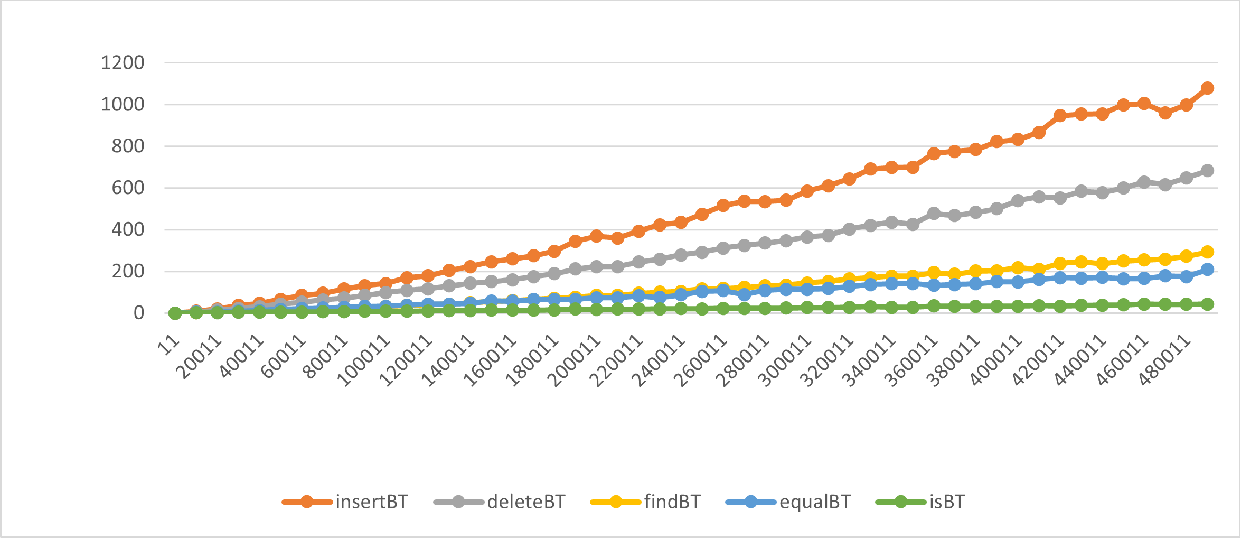
\includegraphics[width=0.9\columnwidth] {ZeitAvg.pdf}
    \end{center}

    \subsubsection{Einstellungen}
    Die Folgenden Einstellungen wurden bei der Messung verwendet:
    \begin{itemize}
        \item 0 Startelemente
        \item 1000 Elemente Schrittgröße
        \item 20 Schritte
        \item Mitteln über 5 Messungen
    \end{itemize}
    
    \subsubsection{Ergebnisse}
    

    
        \paragraph{InsertBT}
        
        Bei InsertBT ist die längste Laufzeit zu erkennen, da wir den Baum zum Anhängen immer bis zum Ende durchlaufen müssen. Außerdem ist bei einer höheren Elementanzahl ein Anstieg der Steigung zu erkennen.
        Dies könnte auf eine höhere Laufzeit als linear hindeuten.
        Erwartet war eine logarithmische Laufzeit. Demnach liegen wir unter den Erwartungen. 

        \paragraph{DeleteBT}  
        
        DeleteBT hat bei zufälligen Elementen eine dezent kürzere Laufzeit als InsertBT, da wir zum Entfernen eines Elementes nicht zwangsläufig bis zum Ende Laufen müssen.
        Falls jedoch im Knoten des zu löschenden Elements sowohl ein linker, als auch einen rechter Teilbaum existiert, muss der Baum bis zum größten Element des linken Teilbaums traversiert werden, um das Ersatzelement zu finden. Hier lässt sich ein linearer Anstieg erkennen. 
        Dies entspricht demnach dem erwarteten Worst-Case mit einer linearen Komplexität.

        \paragraph{FindBT}
        
        FindBT hat eine deutlich kürzere Laufzeit als DeleteBT und InsertBT, da der Baum in jedem Fall nur bis zum gesuchten Element traversiert wird. 
        Hier haben wir also eine deutlich flachere Kurve. Das könnte auf eine logarithmische Laufzeit hindeuten, wie im Entwurf erwartet. 

        \paragraph{EqualBT}
        
        Auch EqualBT hat eine sehr flache Kurve. Logarithmische Laufzeit. Schneller als erwartet.

        \paragraph{IsBT}
        
        IsBT hat mit Abstand die kürzeste Laufzeit von allen Funktionen. Erwartet war eine lineare Laufzeit, wir liegen also deutlich über unseren Erwartungen.

    \subsection{Aufsteigend und Absteigend}\label{subsec:average}

    \begin{center}
        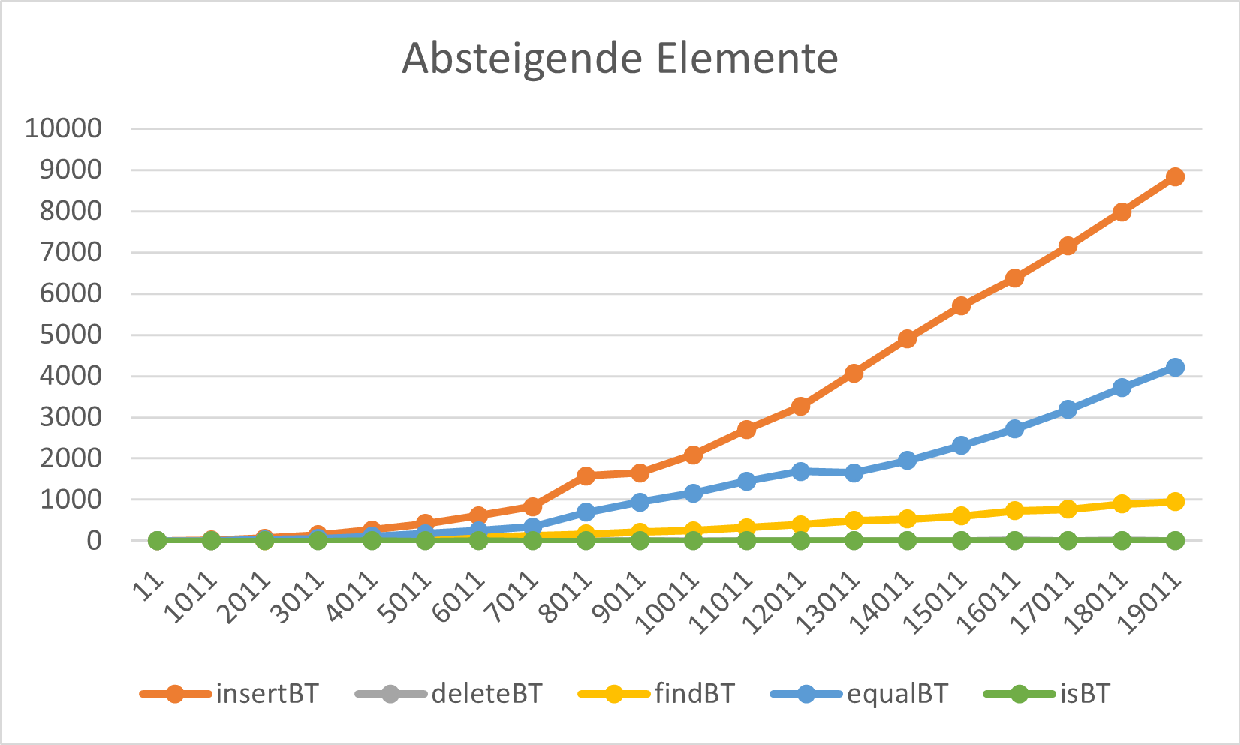
\includegraphics[width=0.9\columnwidth] {ZeitAb.pdf}
    \end{center}
    \begin{center}
        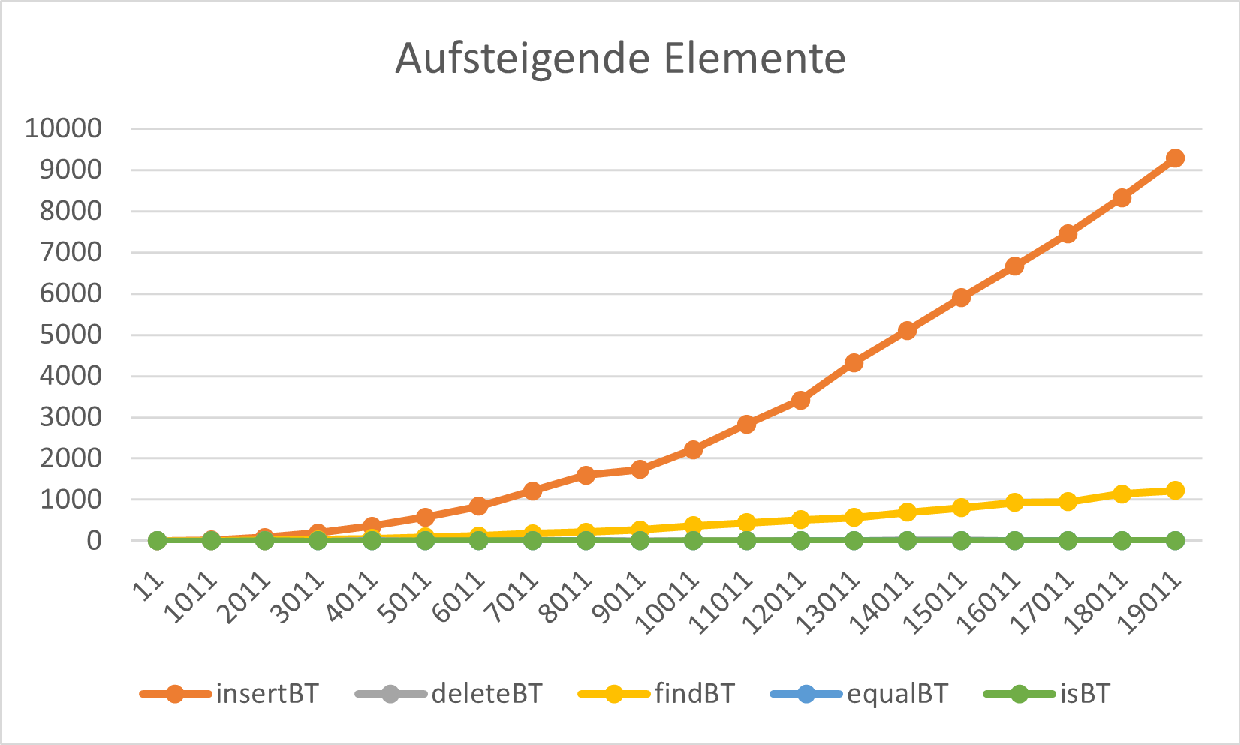
\includegraphics[width=0.9\columnwidth] {ZeitAuf.pdf}
    \end{center}

    \subsubsection{Einstellungen}
    Die Folgenden Einstellungen wurden bei der Messung verwendet:
    \begin{itemize}
        \item 0 Startelemente
        \item 10000 Elemente Schrittgröße
        \item 50 Schritte
        \item Mitteln über 10 Messungen
    \end{itemize}

    \subsubsection{Ergebnisse}
    \paragraph{InsertBT}
        
    Bei InsertBT vermuten wir sowohl mit absteigenden Elementen, als auch mit aufsteigenden Elementen eine quadratische Laufzeit, da ein starker Anstieg der Steigung bei einer höheren Elementanzahl sichtbar ist.

    \paragraph{FindBT}
        
    FindBT besitzt wie erwartet eine sehr flache Kurve.
    Unterschiede zum Average-Case sollte es hier nicht geben. 
    In beiden Fällen wird der Baum bis zum gesuchten Element traversiert.

    \paragraph{DeleteBT}  
    
    Die Laufzeit von DeleteBT hat bei den Extremfällen eine deutlich flachere Kurve, als bei zufällig angeordneten Elementen. Wir gehen davon aus, dass dies nicht die tatsächliche Laufzeit wiederspiegelt. 
    Erwartet war die gleiche Laufzeit wie bei FindBT, da in einem Baum mit aufsteigenden bzw. absteigenden Element stets nur bis zum zu löschenden Element traversiert werden muss.
    Dies könnte sowohl an nicht gefundenen Fehlern der Implementation, als auch an Fehlern in der Messung selbst liegen.


        
    \paragraph{IsBT, EqualBT}  
    
    IsBT und EqualBT sollten bei beiden Grenzfällen die gleiche Laufzeit besitzen wie bei einer zufälligen Anordnung, da alle Knoten durchlaufen werden müssen. Dies lässt sich nicht in den Ergebnissen erkennen, da das gleiche Problem auftritt wie bei DeleteBT.

\end{document}
